%% LyX 1.6.4 created this file.  For more info, see http://www.lyx.org/.
%% Do not edit unless you really know what you are doing.
\documentclass[english]{article}
\usepackage[T1]{fontenc}
\usepackage[latin9]{inputenc}
\usepackage{amsmath}
\usepackage{graphicx}
\usepackage{amssymb}

\makeatletter
\@ifundefined{showcaptionsetup}{}{%
 \PassOptionsToPackage{caption=false}{subfig}}
\usepackage{subfig}
\makeatother

\usepackage{babel}

\begin{document}

\section{Design of a new real-time length-based contention manager with priority
(RTLCM-P)}

For both G-EDF/EDF CM (ECM) and G-RMA/RMA CM (RCM), $s_{i}^{k}(\theta)$
can be totally repeated if $s_{j}^{l}(\theta)$- which belongs to
a higher priority task $T_{j}$ than $T_{i}$- interferes with $s_{i}^{k}(\theta)$
at the end of its execution, while $s_{i}^{k}(\theta)$ is just about
to commit. So, the RTLCM-P  takes the remaining length of $s_{i}^{k}(\theta)$,
as well as $len(s_{j}^{l}(\theta))$, into consideration when deciding
which transaction should abort. The RTLCM-P  can also consider priority
of the conflicting tasks.


\subsection{\label{sec 9.1}Design rationale of RTLCM-P }

It is assumed that $len(s_{j}^{l}(\theta))=c_{m}len(s_{i}^{k}(\theta))$,
where $c_{m}\in]0,\infty[$, to cover all possible lengths of $s_{j}^{l}(\theta)$.
The idea is to reduce the opportunity of abortion of $s_{i}^{k}(\theta)$
when it is close to commit when it is interfered, and $len(s_{j}^{l}(\theta))$
is large. This abortion opportunity increases more and more as $s_{i}^{k}(\theta)$
gets closer to its end of execution, or $len(s_{j}^{l}(\theta))$
gets larger. On the other side, as $s_{i}^{k}(\theta)$ is early interfered,
or $len(s_{j}^{l}(\theta))$ is small compared to the remaining length
of $s_{i}^{k}(\theta)$. To decide whether $s_{i}^{k}(\theta)$ should
abort or not, we use a threshold value $\psi\in[0,1]$, that determines
the length percentage of $s_{i}^{k}(\theta)$-$\alpha_{max}^{jl}$-
below which $s_{i}^{k}(\theta)$ will abort due to $s_{j}^{l}(\theta)$.
If abort percent (abort opportunity) is 0, this means {}``do not
abort'', but if it is 1, this means {}``abort''. Any value between
them means {}``to aport with an opportunity equal to this value''.
The behaviour of RTLCM-P  is shown in Figure \ref{fig16}.

%
\begin{figure}
\begin{centering}
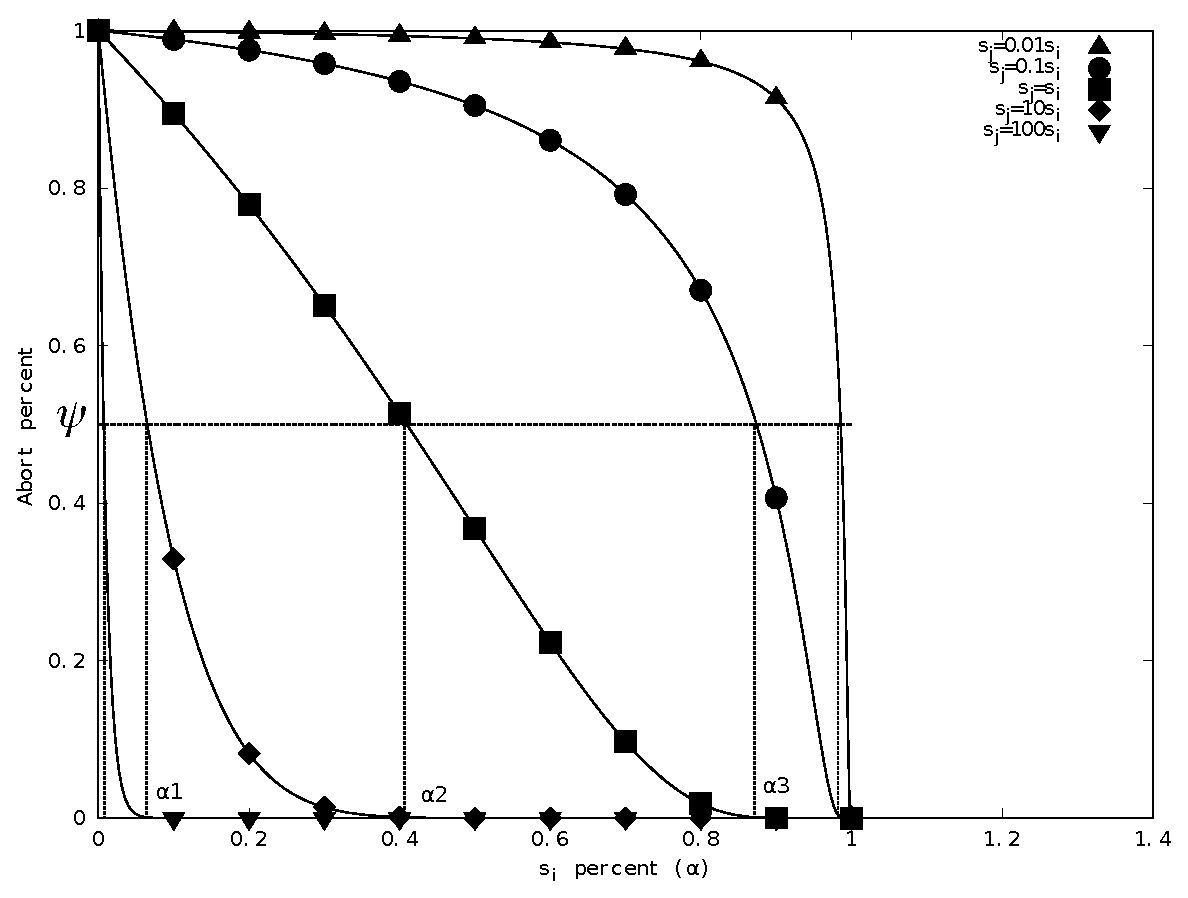
\includegraphics[scale=0.6]{figures/figure16}
\par\end{centering}

\caption{\label{fig16}Interference of $s_{i}^{k}(\theta)$ by various length
$s_{j}^{l}(\theta)$}

\end{figure}


Figure \ref{fig16} represents five different lengths of $s_{j}^{l}(\theta)$
interfering with $s_{i}^{k}(\theta)$ at all points of $s_{i}^{k}(\theta)$.
For a specific curve (which means a specific length for $s_{j}^{l}(\theta)$),
$\psi$ value determines the percentage of $len(s_{i}^{k}(\theta))$
above which $s_{i}^{k}(\theta)$ will be aborted. For example, for
$len(s_{j}^{l}(\theta))=0.1\times len(s_{i}^{k}(\theta))$, $s_{i}^{k}(\theta)$
will be aborted by $s_{j}^{l}(\theta)$ if the latter interferes with
$s_{i}^{k}(\theta)$ no later than $s_{i}^{k}(\theta)$ reaches $\alpha3$
percentages of its length. After that, $s_{j}^{l}(\theta)$ will have
to retry. As $len(s_{j}^{k}(\theta))$ decreases, the opportunity
that it will abort $s_{i}^{k}(\theta)$ at a higher percentage $\alpha_{max}$
increases, as $\alpha3>\alpha2>\alpha1$. The chosen function to represent
different curves in Figure \ref{fig16} is \begin{equation}
f(c_{m},\alpha)=e^{\frac{-c_{m}\alpha}{1-\alpha}}\label{eq49}\end{equation}
where $c_{m}$ is fixed for a specific curve, but $\alpha$ changes
along each curve. This function acheives the desired requirements
that the abortion opportunity is reduced as $s_{i}^{k}(\theta)$ gets
closer to its end of execution (as $\alpha\rightarrow1,\, f(c_{m},1)\rightarrow0$),
or as the length of the conflicting transaction is large (as $c_{m}\rightarrow\infty,\, f(\infty,\alpha)\rightarrow0$).
Meanwhile, this abort opportunity is increased as $s_{i}^{k}(\theta)$
is interfered closer to its release (as $\alpha\rightarrow0,\, f(c_{m},0)\rightarrow1$),
or as length of conlicting transaction decreases (as $c_{m}\rightarrow0,\, f(0,\alpha)\rightarrow1$).
It should be noted that all lengths of $s_{i}^{k}(\theta)$ are normalized
to the same unit length, this way different values of $s_{j}^{l}(\theta)$
intercept different lengths of $s_{i}^{k}(\theta)$ at the same percentage
$\alpha_{max}^{jl}$ (the $\alpha$ value the corresponds the threshold
value $\psi$), but the actual length of interception for different
lengths of $s_{i}^{k}(\theta)$ differ according to $len(s_{i}^{k}(\theta))$
(i.e., let $len(s_{i}^{k}(\theta))\ne len(s_{i}^{k+1}(\theta))$,
then for one $s_{j}^{l}(\theta)$, both $s_{i}^{k}(\theta)$ and $s_{i}^{k+1}(\theta)$
will be intercepted at the same value $\alpha_{max}^{jl}$, but $\alpha_{max}len(s_{i}^{k}(\theta))$
differs from $\alpha_{max}len(s_{i}^{k+1}(\theta))$). This normalization
of different lengths of $s_{i}^{k}(\theta)$ is done to simplify calculations.

$s_{j}^{l}(\theta)$ belongs to a higher priority task than $s_{i}^{k}(\theta)$.
If $s_{j}^{l}(\theta)$ starts before or at the same start time of
$s_{i}^{k}(\theta)$, then $s_{i}^{k}(\theta)$ will have to abort
and retry until $s_{j}^{l}(\theta)$ finishes execution. But if $s_{j}^{l}(\theta)$
starts after $s_{i}^{k}(\theta)$, then the comparison illustrated
in Section \ref{sec 9.1} will be applied.

Let $s_{j}^{l}(\theta)$ interferes with $s_{i}^{k}(\theta)$ at $\alpha_{max}^{jl}$
percentage to acheive the threashold value $\psi$, then the maximum
retrial cost of $s_{i}^{k}(\theta)$ due to $s_{j}^{l}(\theta)$ is
\begin{equation}
\alpha_{max}^{jl}len(s_{i}^{k}(\theta))+len(s_{j}^{l}(\theta))\label{eq47}\end{equation}
because if $s_{j}^{l}(\theta)$ interferes with $s_{i}^{k}(\theta)$
at a $\Upsilon$ percentage, where $\Upsilon<\alpha_{max}^{jl}$,
then the maximum retrial cost of $s_{i}^{k}(\theta)$ will be $\Upsilon len(s_{i}^{k}(\theta))+len(s_{j}^{l}(\theta))$
which is lower than that calculated in equation (\ref{eq47}). And
if $s_{j}^{l}(\theta)$ interferes with $s_{i}^{k}(\theta)$ after
$\alpha_{max}^{jl}$ percentage, then $s_{i}^{k}(\theta)$ will not
abort.

It should be noted that a higher priority task, $T_{j}$, can be blocked
by a lower priority one, $T_{i}$, if $s_{j}^{l}(\theta)$ interferes
with $s_{i}^{k}(\theta)$ after the the $\alpha_{max}^{jl}$ percentage.
This blocking time of $T_{j}$, due to $s_{i}^{k}(\theta)$ and $s_{j}^{l}(\theta)$,
is upper bounded by \begin{equation}
(1-\alpha_{max}^{jl})len(s_{i}^{k}(\theta))\label{eq48}\end{equation}



\subsubsection{Response time of G-EDF/RTLCM-P}

By applying the same analogy used to derive equation (\ref{eq50}),
we find that $RC(T_{i})$ can be upper bounded by assuming each conflicting
atomic section, $s_{j}^{l}(\theta)$, causing a retry to the maximum
length atomic section that accesses object $\theta$, and this retry
will be $len(s_{j}^{l}(\theta))+\alpha_{max}^{jl}len(s_{max}(\theta))$,
where $\alpha_{max}^{jl}$ is the maximum percentage of $len(s_{max}(\theta))$
at which $s_{j}^{l}(\theta)$ forces $s_{max}(\theta)$ to retry.
But the subtracted $s_{max}(\theta)$ in equation (\ref{eq50}) will
be replaced by $\alpha_{max}^{*}s_{max}(\theta)$ where $\alpha_{max}^{*}=min_{\forall j,\forall l}\{\alpha_{max}^{jl}\}$,
because we are calculating the worst case retry cost, so the minimum
percentage of $len(s_{max}(\theta))$ should be the one to subtract.
Also, $s_{i_{max}}(\theta)$ is replaced by $\hat{\alpha}_{max}s_{i_{max}}(\theta)$
where $\hat{\alpha}_{max}$ is the maximum percentage of $len(s_{i_{max}}(\theta))$
at which any of the conflicting atomic sections will enforce $s_{i_{max}}(\theta)$
to retry. So, equation (\ref{eq50}) will be 

\begin{eqnarray}
RC(t(T_{i})) & \le & \sum_{\theta\in\theta_{i}}((\sum_{T_{j}\in\gamma(\theta)}(\lceil\frac{t(T_{i})}{t(T_{j})}\rceil\sum_{\forall s_{j}^{l}(\theta)}len(s_{j}^{l}(\theta))+\alpha_{max}^{jl}len(s_{max}(\theta))))\nonumber \\
 &  & -\alpha_{max}^{*}len(s_{max}(\theta))+\hat{\alpha}_{max}len(s_{i_{max}}(\theta)))\label{eq50}\end{eqnarray}


The same way, equation (\ref{eq4}) will be \begin{eqnarray}
RC(t(T_{i})) & \le & \sum_{\theta\in\theta_{i}}((\sum_{T_{j}\in\gamma(\theta)}(\lceil\frac{t(T_{i})}{t(T_{j})}\rceil\sum_{\forall s_{j}^{l}(\theta)}len(s_{j}^{l}(\theta))+\alpha_{max}^{jl}len(s_{max}^{*}(\theta))))\nonumber \\
 &  & -\alpha_{max}^{*}len(\bar{s}_{max}(\theta))+\hat{\alpha}_{max}len(s_{i_{max}}(\theta)))\label{eq51}\end{eqnarray}
and $RC(T_{i})$ will be calculated as in equation (\ref{eq5}) but
with using equations (\ref{eq50},\ref{eq51}) for each object $\theta$
instead of equations (\ref{eq3},\ref{eq4}) to get equation (\ref{eq53}).

\begin{equation}
RC(t(T_{i}))\le\sum_{\theta\in\theta_{i}}min\begin{cases}
\begin{cases}
((\sum_{T_{j}\in\gamma(\theta)}(\lceil\frac{t(T_{i})}{t(T_{j})}\rceil\sum_{\forall s_{j}^{l}(\theta)\in s_{j}(\theta)}len(s_{j}^{l}(\theta))+\alpha_{max}^{jl}len(s_{max}(\theta))))\\
\alpha_{max}^{*}len(s_{max}(\theta))+\hat{\alpha}_{max}len(s_{i_{max}}(\theta)))\end{cases}\\
\\\begin{cases}
((\sum_{T_{j}\in\gamma(\theta)}(\lceil\frac{t(T_{i})}{t(T_{j})}\rceil\sum_{\forall s_{j}^{l}(\theta)\in s_{j}(\theta)}len(s_{j}^{l}(\theta))+\alpha_{max}^{jl}len(s_{max}^{*}(\theta))))\\
-\alpha_{max}^{*}len(\bar{s}_{max}(\theta))+\hat{\alpha}_{max}len(s_{i_{max}}(\theta)))\end{cases}\\
\\\end{cases}\label{eq53}\end{equation}


To get a tighter retry cost, the same rationale of equation (\ref{eq15})
can be used to get equation (\ref{eq52})

\begin{equation}
RC(t(T_{i}))\le\sum_{\theta\in\theta_{i}}min\begin{cases}
\begin{cases}
((\sum_{T_{j}\in\gamma(\theta)}(\sum_{\forall s_{j}^{l^{*}}(\theta)}len(s_{j}^{l^{*}}(\theta))+\alpha_{max}^{jl}len(s_{max}(\theta)))+\\
(\lfloor\frac{t(T_{i})}{t(T_{j})}\rfloor\sum_{\forall s_{j}^{l}(\theta)}len(s_{j}^{l}(\theta))+\alpha_{max}^{jl}len(s_{max}(\theta))))-\alpha_{max}^{*}len(s_{max}(\theta))+\hat{\alpha}_{max}len(s_{i_{max}}(\theta)))\end{cases}\\
\\\begin{cases}
((\sum_{T_{j}\in\gamma(\theta)}(\sum_{\forall s_{j}^{l^{*}}(\theta)}len(s_{j}^{l^{*}}(\theta))+\alpha_{max}^{jl}len(s_{max}^{*}(\theta)))+\\
(\lceil\frac{t(T_{i})}{t(T_{j})}\rceil\sum_{\forall s_{j}^{l}(\theta)}len(s_{j}^{l}(\theta))+\alpha_{max}^{jl}len(s_{max}^{*}(\theta))))-\alpha_{max}^{*}len(\bar{s}_{max}(\theta))+\hat{\alpha}_{max}len(s_{i_{max}}(\theta)))\end{cases}\\
\\\end{cases}\label{eq52}\end{equation}


As was said in Section \ref{sec 9.1}, $T_{i}$ can be blocked by
a lower priority task $T_{h}$, if an atomic section of $T_{i}$,
$s_{i}^{k}(\theta)$ interferes with one of the atomic sections in
$T_{h}$,$s_{h}^{z}(\theta)$, after the maximum allowed percentage
of $len(s_{h}^{z}(\theta))$, then, $s_{i}^{k}(\theta)$ will abort
and retry until $s_{h}^{z}(\theta)$ finishes.

Let $T_{i}^{x}$ be the studied instance of $T_{i}$. For the case
of G-EDF, there can be at most only one instance of $T_{h}$, $T_{h}^{v}$,
during $t(T_{i})$, that can have a lower priority (larger absolute
deadline) than $T_{i}^{x}$. As it was shown that the worst interference
pattern of $T_{h}$ to $T_{i}$ occurs when the absolute deadline
of one instance of $T_{h}$, $T_{h}^{p}$, coincides with the absolute
deadline of $T_{i}^{x}$. This means that the $T_{h}^{p+1}$ will
be the first instance of $T_{h}$ with lower priority than $T_{i}^{x}$,
but $T_{h}^{p+1}$ will be released after $d(T_{i}^{x})$, so it will
not block $T_{i}^{x}$. So, to get the instance of $T_{h}$ that can
block $T_{i}^{x}$, the worst interference pattern is shifted a little
to the right, as shown in Figure \ref{fig17-b}, so that $T_{h}^{p}$
will be a carried-out job that can block $T_{i}^{x}$.

%
\begin{figure}
\subfloat[\label{fig17-a}No blocking to $T_{i}$]{\begin{centering}
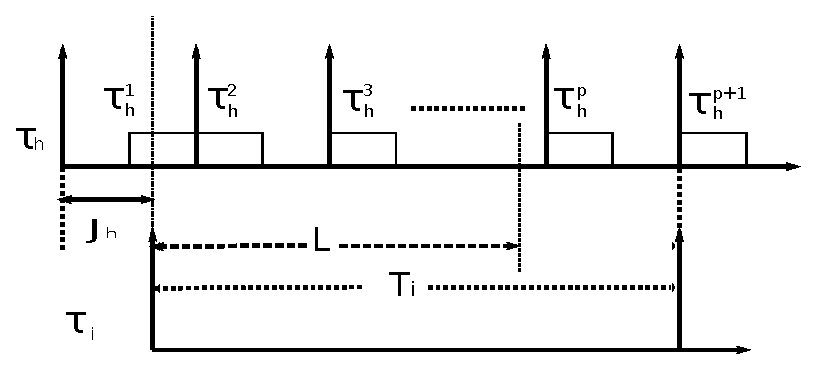
\includegraphics[scale=0.5]{figures/figure17-a}
\par\end{centering}

}

\subfloat[\label{fig17-b}Blocking to $T_{i}$ by $T_{h}^{p}$]{\begin{centering}
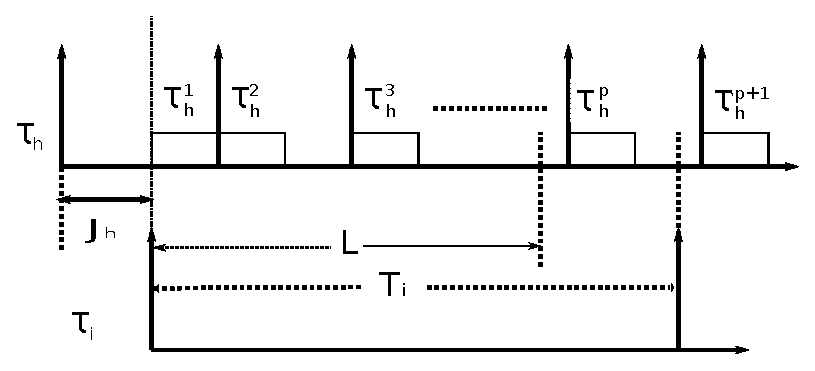
\includegraphics[scale=0.5]{figures/figure17-b}
\par\end{centering}

}

\caption{\label{fig17}Interference to $T_{i}$ by higher and lower priority
tasks}

\end{figure}
So, we have two cases for $T_{i}$. The first one shown in Figure
\ref{fig17-a} which represents the worst case interference pattern
of $T_{h}$ to $T_{i}$. $T_{i}$ does not suffer blocking because
$T_{h}^{p+1}$ is released after the absolute deadline of $T_{i}^{x}$,
but $T_{i}^{x}$ sufferes only from retry cots due to instances $T_{h}^{1}$
to $T_{h}^{p}$, and the retry cost is given in equation (\ref{eq57})
and its tighter form (\ref{eq52}). The other case is shown in Figure
\ref{fig17-b}, where the interference pattern in Figure \ref{fig17-a}
is shifted to the right, so priority of $T_{h}^{p}$ is lower than
that of $T_{i}^{x}$. So, $T_{i}^{x}$ suffers retry cost due to instances
$T_{h}^{1}$ to $T_{h}^{p-1}$, and suffers blocking (as in equation
(\ref{eq48})) due to instance $T_{h}^{p}$. Any further instance
than $T_{h}^{p}$ cannot block $T_{i}^{x}$ because they all start
after $d(T_{i}^{x})$. The retry and blocking costs of $T_{i}$ can
be obtained by modifying equation (\ref{eq57}) to include only instances
$T_{h}^{1}$ to $T_{h}^{p-1}$ in the retry cost, and $T_{h}^{p}$
in the blocking cost. But as priority of $T_{i}^{x}$ is higher than
that of $T_{h}^{p}$, then any atomic section $s_{i}^{y}(\theta)$
in $T_{i}^{x}$ can be blocked by only one conflicting atomic section,
$s_{h}^{z}(\theta)$, of $T_{h}^{p}$. This is because after $s_{h}^{z}(\theta)$,
$s_{i}^{y}(\theta)$ will at most start at the same time as any further
conflicting atomic section in $T_{h}^{z}$, and as $s_{i}^{y}(\theta)$
belongs to a higher priority task, then the RTLCM-P -P will allow
it to commit first. On the other hand, one atomic section in $T_{h}$,
$s_{h}^{z}(\theta)$, can block multiple atomic sections in $T_{i}$
because any atomic section with a suitable length in any other task
can enforce $s_{h}^{z}(\theta)$ to retry multiple times, causing
multiple atomic sections in $T_{i}$ to interfer with $s_{h}^{z}(\theta)$.
So, the worst case for blocking of $T_{i}^{x}$ by $T_{h}^{p}$ occurs
if all atomic sections in $T_{i}^{x}$ that access a specific object
$\theta$ are blocked by the maximum-length atomic section in $T_{h}^{p}$
as shown in equation (\ref{eq55}).\begin{equation}
B_{ih}\le\sum_{\forall s_{i}^{y}(\theta)}(1-\alpha_{max}^{iy})len(s_{h_{max}}(\theta))\label{eq55}\end{equation}
where $\alpha_{max}^{iy}$ is the maximum percentage of $len(s_{h_{max}}(\theta))$
after which $s_{i}^{y}(\theta)$ will be enforced to abort and retry.

Thus, equation (\ref{eq53}) and its tighter form (\ref{eq52}) can
be modified to equation (\ref{eq57}) that includes the effect of
blocking. But as equation (\ref{eq57}) includes both retry and blocking
cost, it will be called $BR(T_{i})$.

\begin{equation}
BR(t(T_{i}))\le\sum_{\theta\in\theta_{i}}min\begin{cases}
\begin{cases}
((\sum_{T_{h}\in\gamma_{(\theta)}}(B_{ih}+\lfloor(\frac{t(T_{i})}{t(T_{h})}\rfloor\sum_{\forall s_{h}^{z}(\theta)}len(s_{h}^{z}(\theta))+\alpha_{max}^{hz}len(s_{max}(\theta))))\\
-\alpha_{max}^{*}len(s_{max}(\theta))+\hat{\alpha}_{max}len(s_{i_{max}}(\theta)))\end{cases}\\
\\\begin{cases}
((\sum_{T_{h}\in\gamma_{(\theta)}}(B_{ih}+\lfloor\frac{t(T_{i})}{t(T_{h})}\rfloor\sum_{\forall s_{h}^{z}(\theta)}len(s_{h}^{z}(\theta))+\alpha_{max}^{hz}len(s_{max}^{*}(\theta))))\\
-\alpha_{max}^{*}len(\bar{s}_{max}(\theta))+\hat{\alpha}_{max}len(s_{i_{max}}(\theta)))\end{cases}\\
\\\end{cases}\label{eq54}\end{equation}
To get the total effect of $T_{h}$ on $T_{i}$, we take the maximum
cost between retry without blocking and retry with blocking that each
$T_{h}^{p}$ imposes on $T_{i}^{x}$. But as equation (\ref{eq54})
calculates costs depending on each object $\theta$, then a task $T_{h}$
may produce a maximum effect on $T_{i}$ for a specific object $\theta_{1}$
if it induces no blocking, but for another object $\theta_{2}$, it
induces blocing on $T_{i}$ to get the maximum cost, but $T_{h}$
cannot be in the two positions for the same $T_{i}$. This why equation
(\ref{eq54}) should be calculated based on each task $T_{h}$, not
on each object $\theta\in\theta_{i}$. This modification also applies
to equations (\ref{eq53},\ref{eq52}). Thus, the final cost imposed
by all $T_{h}$ on $T_{i}$ (this cost will be called $CO(t(T_{i}))$)
will be calculated by equation (\ref{eq56}) depending on equations
(\ref{eq53},\ref{eq54}), or by equation (\ref{eq57}) depending
on equation (\ref{eq52}) (the tighter form of equation (\ref{eq53}))
and equation (\ref{eq54}).

\begin{equation}
CO(t(T_{i}))\le\sum_{T_{h}\in\gamma_{i}}max\begin{cases}
min\begin{cases}
\begin{cases}
((\sum_{\theta\in\theta_{i}\wedge\theta_{h}}(\lceil\frac{t(T_{i})}{t(T_{h})}\rceil\sum_{\forall s_{h}^{z}(\theta)}len(s_{h}^{z}(\theta))+\alpha_{max}^{hz}len(s_{max}(\theta))))\\
-\alpha_{max}^{*}len(s_{max}(\theta))+\hat{\alpha}_{max}len(s_{i_{max}}(\theta)))\end{cases}\\
\begin{cases}
((\sum_{\theta\in\theta_{i}\wedge\theta_{h}}(\lceil\frac{t(T_{i})}{t(T_{h})}\rceil\sum_{\forall s_{h}^{z}(\theta)}len(s_{h}^{z}(\theta))+\alpha_{max}^{hz}len(s_{max}^{*}(\theta))))\\
-\alpha_{max}^{*}len(\bar{s}_{max}(\theta))+\hat{\alpha}_{max}len(s_{i_{max}}(\theta)))\end{cases}\end{cases}\\
min\begin{cases}
\begin{cases}
((\sum_{\theta\in\theta_{i}\wedge\theta_{h}}(B_{ih}+\lfloor(\frac{t(T_{i})}{t(T_{h})}\rfloor\sum_{\forall s_{h}^{z}(\theta)}len(s_{h}^{z}(\theta))+\alpha_{max}^{hz}len(s_{max}(\theta))))\\
-\alpha_{max}^{*}len(s_{max}(\theta))+\hat{\alpha}_{max}len(s_{i_{max}}(\theta)))\end{cases}\\
\begin{cases}
((\sum_{\theta\in\theta_{i}\wedge\theta_{h}}(B_{ih}+\lfloor\frac{t(T_{i})}{t(T_{h})}\rfloor\sum_{\forall s_{h}^{z}(\theta)}len(s_{h}^{z}(\theta))+\alpha_{max}^{hz}len(s_{max}^{*}(\theta))))\\
-\alpha_{max}^{*}len(\bar{s}_{max}(\theta))+\hat{\alpha}_{max}len(s_{i_{max}}(\theta)))\end{cases}\end{cases}\end{cases}\label{eq56}\end{equation}


\begin{equation}
CO(t(T_{i}))\le\sum_{T_{h}\in\gamma_{i}}max\begin{cases}
min\begin{cases}
\begin{cases}
((\sum_{\theta\in\theta_{i}\wedge\theta_{h}}(\sum_{\forall s_{h}^{z^{*}}(\theta)}len(s_{h}^{z^{*}}(\theta))+\alpha_{max}^{hz}len(s_{max}(\theta)))+\\
(\lfloor\frac{t(T_{i})}{t(T_{h})}\rfloor\sum_{\forall s_{h}^{z}(\theta)}len(s_{h}^{z}(\theta))+\alpha_{max}^{hz}len(s_{max}(\theta))))-\alpha_{max}^{*}len(s_{max}(\theta))+\hat{\alpha}_{max}len(s_{i_{max}}(\theta)))\end{cases}\\
\begin{cases}
((\sum_{\theta\in\theta_{i}\wedge\theta_{h}}(\sum_{\forall s_{h}^{z^{*}}(\theta)}len(s_{h}^{z^{*}}(\theta))+\alpha_{max}^{hz}len(s_{max}^{*}(\theta)))+\\
(\lceil\frac{t(T_{i})}{t(T_{h})}\rceil\sum_{\forall s_{h}^{z}(\theta)}len(s_{h}^{z}(\theta))+\alpha_{max}^{hz}len(s_{max}^{*}(\theta))))-\alpha_{max}^{*}len(\bar{s}_{max}(\theta))+\hat{\alpha}_{max}len(s_{i_{max}}(\theta)))\end{cases}\end{cases}\\
min\begin{cases}
\begin{cases}
((\sum_{\theta\in\theta_{i}\wedge\theta_{h}}(B_{ih}+\lfloor(\frac{t(T_{i})}{t(T_{h})}\rfloor\sum_{\forall s_{h}^{z}(\theta)}len(s_{h}^{z}(\theta))+\alpha_{max}^{hz}len(s_{max}(\theta))))\\
-\alpha_{max}^{*}len(s_{max}(\theta))+\hat{\alpha}_{max}len(s_{i_{max}}(\theta)))\end{cases}\\
\begin{cases}
((\sum_{\theta\in\theta_{i}\wedge\theta_{h}}(B_{ih}+\lfloor\frac{t(T_{i})}{t(T_{h})}\rfloor\sum_{\forall s_{h}^{z}(\theta)}len(s_{h}^{z}(\theta))+\alpha_{max}^{hz}len(s_{max}^{*}(\theta))))\\
-\alpha_{max}^{*}len(\bar{s}_{max}(\theta))+\hat{\alpha}_{max}len(s_{i_{max}}(\theta)))\end{cases}\end{cases}\end{cases}\label{eq57}\end{equation}


Costs of $T_{i}$ can be calculated over an interval $L(T_{i})\le\lfloor\frac{t(T_{i})-c_{h}}{t(T_{h})}\rfloor t(T_{h})+c_{h}$
(which can be deduced from Figure \ref{fig17-b}) to get a tighter
upper bound on response time. But during this $L(T_{i})$ duration,
$T_{i}$ will not be blocked by any instance of $T_{h}$ because of
higher priority of all $T_{h}^{p}$ during $L(T_{i})$ than $T_{i}^{x}$.
If $L(T_{i})$ is increased over its specified limit, then costs of
$T_{i}$ can be calculated by equation (\ref{eq54}) where the last
instance of $T_{h}$ blocks $T_{i}^{x}$, but equation (\ref{eq54})
is already included in $CO(T_{i})$, so there is no need to increase
$L(T_{i})$ over its pecified limit. So, the costs of $T_{i}$ over
$L(T_{i})$ can be obtained from equation (\ref{eq16}), with some
modifications to account for RTLCM-P -P, and this will result in equation
(\ref{eq58})\begin{equation}
RC(L(T_{i}))=\sum_{\theta\in\theta_{i}}min\begin{cases}
\begin{cases}
((\sum_{T_{h}\in\gamma(\theta)}((\lceil\frac{L-c_{h}}{t(T_{h})}\rceil+1)\sum_{\forall s_{h}^{z}(\theta)}len(s_{h}^{z}(\theta))\\
+\alpha_{max}^{hz}len(s_{max}(\theta))))-\alpha_{max}^{*}len(s_{max}(\theta))+\hat{\alpha}_{max}len(s_{i_{max}}(\theta)))\end{cases}\\
\begin{cases}
((\sum_{T_{h}\in\gamma(\theta)}((\lceil\frac{L-c_{h}}{t(T_{h})}\rceil+1)\sum_{\forall s_{h}^{z}(\theta)}len(s_{h}^{z}(\theta))\\
+\alpha_{max}^{hz}len(s_{max}^{*}(\theta))))-\alpha_{max}^{*}len(\bar{s}_{max}(\theta))+\hat{\alpha}_{max}len(s_{i_{max}}(\theta)))\end{cases}\end{cases}\label{eq58}\end{equation}
So, the final costs of $T_{i}$, $CO(T_{i})$, can be calculated by
equation (\ref{eq59}).\begin{equation}
CO(T_{i})=\begin{cases}
RC(L(T_{i})) & if\, L(T_{i})\le\lfloor\frac{t(T_{i})-c_{h}}{t(T_{h})}\rfloor t(T_{h})+c_{h}\\
CO(t(T_{i})) & otherwise\end{cases}\label{eq59}\end{equation}
and response time of $T_{i}$ can be calculated by equation (\ref{eq10})
but $RC(T_{i})$ will be replaced with $CO(T_{i})$.


\subsubsection{\label{sub:Comparison-between-G-EDF/EDF}Comparison between G-EDF/EDF
CM (ECM) and G-EDF/RTLCM-P}

Execution time of each task $T_{i}$ , in G-EDF/RTLCM-P, is inflated
by addingt $CO(T_{i})$ to $c_{i}$, and in ECM, by adding $RC(T_{i})$
to $c_{i}$. Then, total utilization between ECM and G-EDF/RTLCM-P
are compared to know when G-EDF/RTLCM-P will be better as follows
:-

\begin{eqnarray*}
\sum_{\forall T_{i}}\frac{c_{i}+CO(T_{i})}{t(T_{i})} & \le & \sum_{\forall T_{i}}\frac{c_{i}+RC(T_{i})}{t(T_{i})}\\
\sum_{\forall T_{i}}\frac{CO(T_{i})}{t(T_{i})} & \le & \sum_{\forall T_{i}}\frac{RC(T_{i})}{t(T_{i})}\end{eqnarray*}


But the $RC(T_{i})$ is upper bounded by equation (\ref{eq30})\begin{equation}
RC(T_{i})\le\sum_{T_{h}\in\gamma_{i}}(\sum_{\theta\in\theta_{i}\wedge\theta_{h}}(\lceil\frac{t(T_{i})}{t(T_{h})}\rceil\sum_{\forall s_{h}^{z}(\theta)}(2.s_{max})))\label{eq61}\end{equation}
with the same assumptions that $s_{h}^{l}(\theta)$, $s_{max}(\theta)$,
$s_{i_{max}}(\theta)$, $s_{max}^{*}(\theta)$ and $\bar{s}_{max}(\theta)$
are replaced by $s_{max}$. With the same assumptions, $CO(T_{i})$
can also be upper bounded by \begin{equation}
CO(T_{i})\le\sum_{T_{h}\in\gamma_{i}}max\begin{cases}
(\sum_{\theta\in\theta_{i}\wedge\theta_{h}}(\lceil\frac{t(T_{i})}{t(T_{h})}\rceil\sum_{\forall s_{h}^{z}(\theta)}(1+\alpha_{max})s_{max}))\\
(\sum_{\theta\in\theta_{i}\wedge\theta_{h}}((\sum_{\forall s_{i}^{y}(\theta)}(1-\alpha_{max})s_{max})+\lfloor\frac{t(T_{i})}{t(T_{h})}\rfloor\sum_{\forall s_{h}^{z}(\theta)}(1+\alpha_{max})s_{max}))\end{cases}\label{eq62}\end{equation}
where all atomic sections are replaced by $s_{max}$, hence $\alpha$
will be the same for all atomic sections and will be called $\alpha_{max}$.
So, $s_{max}$ and $\alpha_{max}$ are both constants. If $\sum_{\theta\in\theta_{i}\wedge\theta_{h}}\sum_{\forall s_{h}^{z}(\theta)}$
and $\sum_{\theta\in\theta_{i}\wedge\theta_{h}}\sum_{\forall s_{i}^{y}(\theta)}$
are both lower than $\beta_{i,h}$, which is the maximum access number
of all shared objects by both $T_{i}$ and $T_{h}$. So, equation
(\ref{eq61}) will be\begin{equation}
RC(T_{i})\le\sum_{T_{h}\in\gamma_{i}}2\lceil\frac{t(T_{i})}{t(T_{h})}\rceil\beta_{i,h}s_{max}\label{eq63}\end{equation}
and equation (\ref{eq62}) will be \begin{equation}
CO(T_{i})\le\sum_{T_{h}\in\gamma_{i}}max\begin{cases}
\beta_{i,h}\lceil\frac{t(T_{i})}{t(T_{h})}\rceil(1+\alpha_{max})s_{max}\\
((1-\alpha_{max})+\lfloor\frac{t(T_{i})}{t(T_{h})}\rfloor(1+\alpha_{max}))\beta_{i,h}s_{max}\end{cases}\label{eq64}\end{equation}


\textbf{\textit{In case }}$t(T_{i})=a_{ih}t(T_{h})$, then $\lceil\frac{t(T_{i})}{t(T_{h})}\rceil=\lfloor\frac{t(T_{i})}{t(T_{h})}\rfloor=a_{ih}$,
and equation (\ref{eq64}) will be\begin{eqnarray}
CO(T_{i}) & \le & \sum_{T_{h}\in\gamma_{i}}max\begin{cases}
\beta_{i,h}a_{ih}(1+\alpha_{max})s_{max}\\
((1-\alpha_{max})+a_{ih}(1+\alpha_{max}))\beta_{i,h}s_{max}\end{cases}\nonumber \\
 & \le & \sum_{T_{h}\in\gamma_{i}}((1-\alpha_{max})+a_{ih}(1+\alpha_{max}))\beta_{i,h}s_{max}\label{eq65}\end{eqnarray}
and equation (\ref{eq63}) will be \[
RC(T_{i})\le\sum_{T_{h}\in\gamma_{i}}2a_{ih}\beta_{i,h}s_{max}\]
Then, G-EDF/RTLCM-P will give better performance if \[
\sum_{\forall T_{i}}\frac{\sum_{T_{h}\in\gamma_{i}}((1-\alpha_{max})+a_{ih}(1+\alpha_{max}))\beta_{i,h}s_{max}}{t(T_{i})}\le\sum_{\forall T_{i}}\frac{\sum_{T_{h}\in\gamma_{i}}2a_{ih}\beta_{i,h}s_{max}}{t(T_{i})}\]
This inequality is ensured if for each $T_{i}$ and $T_{h}$ \begin{eqnarray*}
(1-\alpha_{max})+a_{ih}(1+\alpha_{max}) & \le & 2a_{ih}\\
1-\alpha_{max} & \le & (1-\alpha_{max})a_{ih}\\
1 & \le & a_{ih}\end{eqnarray*}
As $a_{ih}$ is always greater than or equal to 1, then in case $t(T_{i})=a_{ih}t(T_{h})$,
performance of G-EDF/RTLCM-P is better than that of ECM.

\textbf{\textit{In case }}$t(T_{i})=a_{ih}t(T_{h})+\delta$, then
$\lfloor\frac{t(T_{i})}{t(T_{h})}\rfloor=a_{ih}$ and $\lceil\frac{t(T_{i})}{t(T_{h})}\rceil=a_{ih}+1$,
and equation (\ref{eq64}) will be\begin{eqnarray}
CO(T_{i}) & \le & \sum_{T_{h}\in\gamma_{i}}max\begin{cases}
\beta_{i,h}(a_{ih}+1)(1+\alpha_{max})s_{max}\\
((1-\alpha_{max})+a_{ih}(1+\alpha_{max}))\beta_{i,h}s_{max}\end{cases}\nonumber \\
 & \le & \sum_{T_{h}\in\gamma_{i}}\beta_{i,h}(a_{ih}+1)(1+\alpha_{max})s_{max}\label{eq66}\end{eqnarray}
and equation (\ref{eq63}) will be \[
RC(T_{i})\le\sum_{T_{h}\in\gamma_{i}}2(a_{ih}+1)\beta_{i,h}s_{max}\]
For G-EDF/RTLCM-P to be better than ECM, then\[
\sum_{\forall T_{i}}\frac{\sum_{T_{h}\in\gamma_{i}}\beta_{i,h}(a_{ih}+1)(1+\alpha_{max})s_{max}}{t(T_{i})}\le\sum_{\forall T_{i}}\frac{\sum_{T_{h}\in\gamma_{i}}2(a_{ih}+1)\beta_{i,h}s_{max}}{t(T_{i})}\]
This inequality is assured when for each $T_{i}$ and $T_{h}$\begin{eqnarray*}
(a_{ih}+1)(1+\alpha_{max}) & \le & 2(a_{ih}+1)\\
1+\alpha_{max} & \le & 2\\
\alpha_{max} & \le & 1\end{eqnarray*}
Because $\alpha_{max}$ is always less than or equal to 1, then performance
of G-EDF/RTLCM-P is better or equal to that of ECM for $t(T_{i})=a_{ih}t(T_{h})+\delta$.
So, for all cases, G-EDF/RTLCM-P gives better or equal performance
to that of ECM.


\subsubsection{Comparison between G-EDF/RTLCM-P and retry-loop lock-free algorithm}

\textbf{\textit{In case}} $t(T_{i})=a_{ih}t(T_{h})$, then $CO(T_{i})$
is upper bounded by equation (\ref{eq65}), and retry loop cost is
upper bounded by equation (\ref{eq32}). Total utilization of G-EDF/RTLCM-P
is compared to that of retry-loop lock-free algorithm to determine
which is better as follows :- \begin{eqnarray*}
\sum_{\forall T_{i}}\frac{\sum_{\forall T_{h}\in\gamma_{i}}((1-\alpha_{max})+a_{ih}(1+\alpha_{max}))\beta_{i,h}s_{max}}{t(T_{i})} & \le & \sum_{\forall T_{i}}\frac{\sum_{\forall T_{h}\in\gamma_{i}}(a_{ih}+1).\beta_{i,h}.r_{max}}{t(T_{i})}\end{eqnarray*}
\begin{eqnarray*}
\frac{s_{max}}{r_{max}} & \le & \frac{\sum_{\forall T_{i}}\frac{\sum_{\forall T_{h}\in\gamma_{i}}(a_{ih}+1).\beta_{i,h}}{t(T_{i})}}{\sum_{\forall T_{i}}\frac{\sum_{\forall T_{h}\in\gamma_{i}}((1-\alpha_{max})+a_{ih}(1+\alpha_{max}))\beta_{i,h}}{t(T_{i})}}\\
 & \le & \frac{\sum_{\forall T_{i}}\frac{\sum_{\forall T_{h}\in\gamma_{i}}(a_{ih}+1).\beta_{i,h}}{t(T_{i})}}{\sum_{\forall T_{i}}\frac{\sum_{\forall T_{h}\in\gamma_{i}}(a_{ih}+1)\beta_{i,h}}{t(T_{i})}+\sum_{\forall T_{i}}\frac{\sum_{\forall T_{h}\in\gamma_{i}}(a_{ih}-1)\alpha_{max}\beta_{i,h}}{t(T_{i})}}\\
\therefore\frac{r_{max}}{s_{max}} & \ge & \frac{\sum_{\forall T_{i}}\frac{\sum_{\forall T_{h}\in\gamma_{i}}(a_{ih}+1)\beta_{i,h}}{t(T_{i})}+\sum_{\forall T_{i}}\frac{\sum_{\forall T_{h}\in\gamma_{i}}(a_{ih}-1)\alpha_{max}\beta_{i,h}}{t(T_{i})}}{\sum_{\forall T_{i}}\frac{\sum_{\forall T_{h}\in\gamma_{i}}(a_{ih}+1).\beta_{i,h}}{t(T_{i})}}\\
 & \ge & 1+\frac{\alpha_{max}\sum_{\forall T_{i}}\frac{\sum_{\forall T_{h}\in\gamma_{i}}(a_{ih}-1)\beta_{i,h}}{t(T_{i})}}{\sum_{\forall T_{i}}\frac{\sum_{\forall T_{h}\in\gamma_{i}}(a_{ih}+1).\beta_{i,h}}{t(T_{i})}}\end{eqnarray*}
Since $a_{ih}\ge1\,\therefore\sum_{\forall T_{i}}\frac{\sum_{\forall T_{h}\in\gamma_{i}}(a_{ih}-1)\beta_{i,h}}{t(T_{i})}<\sum_{\forall T_{i}}\frac{\sum_{\forall T_{h}\in\gamma_{i}}(a_{ih}+1).\beta_{i,h}}{t(T_{i})}$, 

$\therefore\,1\le\frac{r_{max}}{s_{max}}\le1+\alpha_{max}$

$\therefore\,\frac{1}{1+\alpha_{max}}\le\frac{s_{max}}{r_{max}}\le1$ 

So, by proper choice of $\alpha_{max}$, $\frac{s_{max}}{r_{max}}$
can be greater than 0.5 (which is greater than ECM), but still lower
or equal to 1. In case $a_{ih}\rightarrow1,\,\therefore\frac{s_{max}}{r_{max}}\le1$,
and in case $a_{ih}\rightarrow\infty,\,\therefore\,\frac{s_{max}}{r_{max}}\le\frac{1}{1+\alpha_{max}}$.
So, as number of tasks sharing resources increases, length of $s_{max}$
relative to $r_{max}$ is reduced to a value that is greater than
0.5 depending on $\alpha_{max}$, and when number of tasks sharing
same resources decreases, length of $s_{max}$ can be as large as
$r_{max}$.

\textbf{\textit{In case }}$t(T_{i})=a_{ih}t(T_{h})+\delta$, then
$CO(T_{i})$ is upper bounded by equation (\ref{eq66}), and comparison
between total utilization of G-EDF/RTLCM-P and retry-loop lock-free
is:-

\begin{eqnarray*}
\sum_{\forall T_{i}}\frac{\sum_{T_{h}\in\gamma_{i}}\beta_{i,h}(a_{ih}+1)(1+\alpha_{max})s_{max}}{t(T_{i})} & \le & \sum_{\forall T_{i}}\frac{\sum_{\forall T_{h}\in\gamma_{i}}(a_{ih}+1).\beta_{i,h}.r_{max}}{t(T_{i})}\end{eqnarray*}
\begin{eqnarray*}
\frac{s_{max}}{r_{max}} & \le & \frac{\sum_{\forall T_{i}}\frac{\sum_{\forall T_{h}\in\gamma_{i}}(a_{ih}+1).\beta_{i,h}}{t(T_{i})}}{\sum_{\forall T_{i}}\frac{\sum_{T_{h}\in\gamma_{i}}\beta_{i,h}(a_{ih}+1)(1+\alpha_{max})}{t(T_{i})}}\\
\therefore\,\frac{r_{max}}{s_{max}} & \ge & \frac{\sum_{\forall T_{i}}\frac{\sum_{T_{h}\in\gamma_{i}}(a_{ih}+1)\beta_{i,h}}{t(T_{i})}}{\sum_{\forall T_{i}}\frac{\sum_{\forall T_{h}\in\gamma_{i}}(a_{ih}+1)\beta_{i,h}}{t(T_{i})}}+\frac{\alpha_{max}\sum_{\forall T_{i}}\frac{\sum_{T_{h}\in\gamma_{i}}(a_{ih}+1)\beta_{i,h}}{t(T_{i})}}{\sum_{\forall T_{i}}\frac{\sum_{\forall T_{h}\in\gamma_{i}}(a_{ih}+1).\beta_{i,h}}{t(T_{i})}}\\
 & \ge & 1+\alpha_{max}\end{eqnarray*}
$\therefore\,1\le\frac{s_{max}}{r_{max}}\le\frac{1}{1+\alpha_{max}}$
for all values of $a_{ih}$, and as in the previous case, by prober
choice of $\alpha_{max}$, length of $s_{max}$ can be higher than
half of $r_{max}$ (which is higher than that of ECM), but it still
cannot exceed length of $r_{max}$.


\subsubsection{Comparison between G-EDF/RTLCM-P and locking protocols}

Total utilization of G-EDF/RTLCM-P is compared against total utilization
of FMLP and OMLP locking protocols. As explained in Section \ref{sub:Comparison-between-FMLP},
blocking time of $T_{i}$ under FMLP is upper bounde by \begin{equation}
B(T_{i})\le|s\_\theta|_{max}\sum_{T_{i}}[(N_{i,s}(m-1)+(1+N_{i,l}).max_{k\ne i}(N_{k,s}.(m-1)+1)+N_{i,l}.(n-1).c1)]/t(T_{i})\label{eq67}\end{equation}
and this blocking time is $O(n(n+m))$.

In case $t(T_{i})=a_{ih}t(T_{h})$, then $CO(T_{i})$ is upper bounded
by equation (\ref{eq65}). By assuming $a_{ih}\le Const1$, where
$Const1$ is the maximum number of instances of any task $T_{h}$
in the period of any other task $T_{i}$, then $CO(T_{i})=O(n^{2})$.
In case $t(T_{i})=a_{ih}t(T_{h})+\delta$, then $CO(T_{i})$ is upper
bounded by equation (\ref{eq66}) which is also $O(n^{2})$.

So, for schedulability of G-EDF/RTLCM-P to be better or equal to that
of FMLP, total utilization of G-EDF/RTLCM-P, whether $t(T_{i})$ is
an integer multiple of $t(T_{h})$ or not, is compared against total
utilization of FMLP to give that \begin{eqnarray*}
\frac{s_{max}}{|s\_\theta|_{max}} & = & \frac{O(n(n+m))}{O(n^{2})}\\
 & = & O(\frac{m}{n})\end{eqnarray*}
As mentioned in Section \ref{sec:Comparison-of-OMLP}, the blocking
time for $T_{i}$ is upper bounded by $2.(m-1).L_{max}\sum_{k=1}^{q}N_{i,k}$
which is $O(m)$, and the total utilization of a task set under OMLP
is $O(nm)$, but the total utilization under G-EDF/RTLCM-P is $O(n^{2})$.
So, by comparing total utilization of G-EDF/RTLCM-P and total utilization
of OMLP, we get\[
\frac{s_{max}}{L_{max}}=O(\frac{m}{n})\]
So, it is clear that G-EDF/RTLCM-P gives the same asymptotic schedulability
performance of ECM compared with locking protocols, and this is natural
as the difference between G-EDF/RTLCM-P and ECM is only when an atomic
section, $s_{h}^{z}(\theta)$, of a higher priority task is allowed
to abort an atomic section, $s_{i}^{l}(\theta)$, of a lower priority
task, while this abortion can happen at any point in the life time
of $s_{i}^{l}(\theta)$ in ECM, it is restricted in G-EDF/RTLCM-P.


\subsubsection{Response time in G-RMA/RTLCM-P}

Because of the fixed priority of G-RMA, all instances of the higher
priority task, $T_{j}$, can interfere with the lower priority task,
$T_{i}$, during $t(T_{i})$. So, blocking is not considered with
higher priority tasks than $T_{i}$, but blocking is considered for
all instances, during $t(T_{i})$, of any task, $T_{h}$, with lower
priority than $T_{i}$. Besides, whether response time is calculated
over all $t(T_{i})$, or over an interval $L<t(T_{i})$, the same
equations for costs of $T_{i}$ and response time will be used because
of fixed priority as shown in equations ().\begin{eqnarray}
CO(L(T_{i})) & = & \sum_{(T_{j}\in\gamma_{i})\wedge(p(T_{j})>p(T_{i}))}((\sum_{\theta\in(\theta_{i}\wedge\theta_{j})}((\lceil\frac{L-c_{j}}{t(T_{j})}\rceil+1).\sum_{\forall s_{j}^{l}(\theta)}len(s_{j}^{l}(\theta))+\alpha_{max}^{jl}len(s_{max}^{j}(\theta))))\nonumber \\
 & - & \alpha_{max}^{*}len(s_{max}^{j}(\theta))+\hat{\alpha}_{max}len(s_{i_{max}}(\theta))\label{eq60}\\
 & + & \sum_{(T_{h}\in\gamma_{i})\wedge(p(T_{h})<p(T_{i}))}\sum_{\theta\in(\theta_{i}\wedge\theta_{h})}((\lceil\frac{L-c_{h}}{t(T_{h})}\rceil+1).\sum_{\forall s_{i}^{y}(\theta)}(1-\alpha_{max}^{iy})len(s_{h_{max}}(\theta)))\nonumber \end{eqnarray}
where $L(T_{i})$ can extend to $t(T_{i})$.

Response time can be calculated by equation (\ref{eq22}) with replacing
$RC(T_{i})$ with $CO(L(T_{i}))$.


\subsubsection{Comparison between G-RMA/RTLCM-P G-RMA/RMA CM (RCM)}

By applying the same assumptions in Section \ref{sub:Comparison-between-G-EDF/EDF},
equation (\ref{eq60}) can be upper bounded by \begin{eqnarray}
CO(L(T_{i})) & \le & \sum_{(T_{j}\in\gamma_{i})\wedge(p(T_{j})>p(T_{i}))}(\sum_{\theta\in(\theta_{i}\wedge\theta_{j})}((\lceil\frac{t(T_{i})}{t(T_{j})}\rceil+1).\sum_{\forall s_{j}^{l}(\theta)}(1+\alpha_{max})len(s_{max})))\label{eq68}\\
 & + & \sum_{(T_{h}\in\gamma_{i})\wedge(p(T_{h})<p(T_{i}))}(\sum_{\theta\in(\theta_{i}\wedge\theta_{h})}((\lceil\frac{t(T_{i})}{t(T_{h})}\rceil+1).\sum_{\forall s_{i}^{y}(\theta)}(1-\alpha_{max})len(s_{max})))\nonumber \end{eqnarray}


if $t(T_{i})=a_{ij}t(T_{j})+\delta_{ij}$, and $t(T_{i})=a_{ih}t(T_{h})+\delta_{ih}$$\therefore$
equation (\ref{eq68}) can will be \begin{eqnarray}
CO(L(T_{i})) & \le & \sum_{(T_{j}\in\gamma_{i})\wedge(p(T_{j})>p(T_{i}))}(\sum_{\theta\in(\theta_{i}\wedge\theta_{j})}((a_{ij}+2).\sum_{\forall s_{j}^{l}(\theta)}(1+\alpha_{max})len(s_{max})))+\nonumber \\
 &  & \sum_{(T_{h}\in\gamma_{i})\wedge(p(T_{h})<p(T_{i}))}(\sum_{\theta\in(\theta_{i}\wedge\theta_{h})}((a_{ih}+2).\sum_{\forall s_{i}^{y}(\theta)}(1-\alpha_{max})len(s_{max})))\nonumber \\
 & \le & \sum_{(T_{j}\in\gamma_{i})\wedge(p(T_{j})>p(T_{i}))}((a_{ij}+2)(1+\alpha_{max})len(s_{max})\beta_{ij})+\nonumber \\
 &  & \sum_{(T_{h}\in\gamma_{i})\wedge(p(T_{h})<p(T_{i}))}((a_{ih}+2)(1-\alpha_{max})len(s_{max})\beta_{ih})\label{eq71}\end{eqnarray}
where $\beta_{ij}$ is the number of access times by $T_{j}$ to shared
resources between $T_{i}$ and $T_{j}$, and $\beta_{ih}$ is the
same but between $T_{i}$ and $T_{h}$.

For RCM, $RC(T_{i})$ is upper bounded by\begin{equation}
RC(T_{i})\le\sum_{(T_{j}\in\gamma_{i})\wedge(p(T_{j})\ge p(T_{i}))}(\lceil\frac{t(T_{i})}{t(T_{j})}\rceil+1)2\beta_{ij}s_{max}\label{eq69}\end{equation}


So, by comparing total utilization of G-RMA/RTLCM-P with that of RCM,
we get \begin{eqnarray*}
\sum_{\forall T_{i}}\frac{\sum_{(T_{j}\in\gamma_{i})\wedge(p(T_{j})>p(T_{i}))}((a_{ij}+2)(1+\alpha_{max})len(s_{max})\beta_{ij})+\sum_{(T_{h}\in\gamma_{i})\wedge(p(T_{h})<p(T_{i}))}((a_{ih}+2)(1-\alpha_{max})len(s_{max})\beta_{ih})}{t(T_{i})}\end{eqnarray*}


\[
\le\sum_{\forall T_{i}}\frac{\sum_{(T_{j}\in\gamma_{i})\wedge(p(T_{j})>p(T_{i}))}(a_{ij}+2)2\beta_{ij}len(s_{max})}{t(T_{i})}\]


By dividing both sides by $len(s_{max})$, then subtracting $\sum_{\forall T_{i}}\frac{\sum_{(T_{j}\in\gamma_{i})\wedge(p(T_{j})>p(T_{i}))}((a_{ij}+2)(1+\alpha_{max})len(s_{max})\beta_{ij})}{t(T_{i})}$
from each side

\begin{eqnarray*}
\therefore & \sum_{\forall T_{i}}\frac{\sum_{(T_{h}\in\gamma_{i})\wedge(p(T_{h})<p(T_{i}))}((a_{ih}+2)(1-\alpha_{max})\beta_{ih})}{t(T_{i})}\\
\le & \sum_{\forall T_{i}}\frac{\sum_{(T_{j}\in\gamma_{i})\wedge(p(T_{j})>p(T_{i}))}((a_{ij}+2)(1-\alpha_{max})\beta_{ij})}{t(T_{i})}\end{eqnarray*}


\begin{equation}
\therefore\sum_{\forall T_{i}}\frac{\sum_{(T_{h}\in\gamma_{i})\wedge(p(T_{h})<p(T_{i}))}((a_{ih}+2)\beta_{ih})}{t(T_{i})}\le\sum_{\forall T_{i}}\frac{\sum_{(T_{j}\in\gamma_{i})\wedge(p(T_{j})>p(T_{i}))}((a_{ij}+2)\beta_{ij})}{t(T_{i})}\label{eq70}\end{equation}


$\sum_{\forall T_{i}}\frac{\sum_{(T_{h}\in\gamma_{i})\wedge(p(T_{h})<p(T_{i}))}((a_{ih}+2)\beta_{ih})}{t(T_{i})}$
results from blocking time suffered by all tasks, while $\sum_{\forall T_{i}}\frac{\sum_{(T_{j}\in\gamma_{i})\wedge(p(T_{j})>p(T_{i}))}((a_{ij}+2)\beta_{ij})}{t(T_{i})}$
results from interference time suffered by all tasks. So, if blocking
time for each task $T_{i}$ is kept lower or equal to interference
time suffered by the same task $T_{i}$, then schedulability performance
of G-RMA/RTLCM-P is better or equal to that of RCM. So, equation (\ref{eq70})
can be checked for each task set, and it applies, G-RMA/RTLCM-P is
used, otherwise, RCM is used. It also appears from equation (\ref{eq70})
that schedulability performance of G-RMA/RTLCM-P compared with RCM
does not depend on the chosen value of $\alpha_{max}$, in contrast
to the case of G-EDF/RTLCM-P.


\subsubsection{Comparison between G-RMA/RTLCM-P and retry-loop lock free algorithm}

$CO(T_{i})$ for G-RMA/RTLCM-P is upper bounded by equation (\ref{eq71})
assuming that $t(T_{i})=a_{ij}t(T_{j})+\delta_{ij}$, and $t(T_{i})=a_{ih}t(T_{h})+\delta_{ih}$
(the case of $t(T_{i})$ being an integer multiple of $t(T_{j})$
and $t(T_{h})$ is not considered here because it will not affect
conclusions). $RC(T_{i})$ for retry-loop lock-free algorithm is upper
bounded by equation (\ref{eq32}) which is re-written here as\begin{equation}
RC(T_{i})=\sum_{T_{v}\in\gamma_{i}}(\lceil\frac{t(T_{i})}{t(T_{v})}\rceil+1)\beta_{iv}r_{max}\label{eq72}\end{equation}
But set of tasks $T_{v}\in\gamma_{i}$ are composed of tasks of higher
priority than $T_{i}$, which are donated as $T_{j}$ in consistence
to the index notation of G-RMA/RTLCM-P, and tasks of lower priority
than $T_{i}$, which are donated as $T_{h}$. So, equation (\ref{eq72})
can be re-written as equation (\ref{eq73}).\begin{equation}
RC(T_{i})=\sum_{(T_{j}\in\gamma_{i})\wedge(p(T_{j})>p(T_{i}))}(\lceil\frac{t(T_{i})}{t(T_{j})}\rceil+1)\beta_{ij}r_{max}+\sum_{(T_{h}\in\gamma_{i})\wedge(p(T_{h})<p(T_{i}))}(\lceil\frac{t(T_{i})}{t(T_{h})}\rceil+1)\beta_{ih}r_{max}\label{eq73}\end{equation}


So, to determine when schedulability performance of G-RMA/RTLCM-P
will be better or equal to that of retry-loop lock-free, we compare
total utilization of both as follows:-\[
\sum_{\forall T_{i}}\frac{\sum_{(T_{j}\in\gamma_{i})\wedge(p(T_{j})>p(T_{i}))}((a_{ij}+2)(1+\alpha_{max})len(s_{max})\beta_{ij})+\sum_{(T_{h}\in\gamma_{i})\wedge(p(T_{h})<p(T_{i}))}((a_{ih}+2)(1-\alpha_{max})len(s_{max})\beta_{ih})}{t(T_{i})}\]


\[
\le\sum_{\forall T_{i}}\frac{\sum_{(T_{j}\in\gamma_{i})\wedge(p(T_{j})>p(T_{i}))}(a_{ij}+2)\beta_{ij}r_{max}+\sum_{(T_{h}\in\gamma_{i})\wedge(p(T_{h})<p(T_{i}))}(a_{ih}+2)\beta_{ih}r_{max}}{t(T_{i})}\]


$\therefore$

\begin{eqnarray}
\frac{s_{max}}{r_{max}} & \le & \frac{\sum_{\forall T_{i}}\frac{\sum_{(T_{j}\in\gamma_{i})\wedge(p(T_{j})>p(T_{i}))}(a_{ij}+2)\beta_{ij}+\sum_{(T_{h}\in\gamma_{i})\wedge(p(T_{h})<p(T_{i}))}(a_{ih}+2)\beta_{ih}}{t(T_{i})}}{\sum_{\forall T_{i}}\frac{\sum_{(T_{j}\in\gamma_{i})\wedge(p(T_{j})>p(T_{i}))}((a_{ij}+2)(1+\alpha_{max})\beta_{ij})+\sum_{(T_{h}\in\gamma_{i})\wedge(p(T_{h})<p(T_{i}))}((a_{ih}+2)(1-\alpha_{max})\beta_{ih})}{t(T_{i})}}\label{eq74}\end{eqnarray}
If $\frac{s_{max}}{r_{max}}$ is kept lower or equal to $\frac{\sum_{\forall T_{i}}\frac{\sum_{(T_{j}\in\gamma_{i})\wedge(p(T_{j})>p(T_{i}))}(a_{ij}+2)\beta_{ij}+\sum_{(T_{h}\in\gamma_{i})\wedge(p(T_{h})<p(T_{i}))}(a_{ih}+2)\beta_{ih}}{t(T_{i})}}{\sum_{\forall T_{i}}\frac{\sum_{(T_{j}\in\gamma_{i})\wedge(p(T_{j})>p(T_{i}))}((a_{ij}+2)(1+\alpha_{max})\beta_{ij})+\sum_{(T_{h}\in\gamma_{i})\wedge(p(T_{h})<p(T_{i}))}((a_{ih}+2)(1+\alpha_{max})\beta_{ih})}{t(T_{i})}}$,
where $1-\alpha_{max}$ in denominator the right hand side of inequality
(\ref{eq74}) is replaced by $1+\alpha_{max}$, then inequality (\ref{eq74})
is ensured because $\frac{\sum_{\forall T_{i}}\frac{\sum_{(T_{j}\in\gamma_{i})\wedge(p(T_{j})>p(T_{i}))}(a_{ij}+2)\beta_{ij}+\sum_{(T_{h}\in\gamma_{i})\wedge(p(T_{h})<p(T_{i}))}(a_{ih}+2)\beta_{ih}}{t(T_{i})}}{\sum_{\forall T_{i}}\frac{\sum_{(T_{j}\in\gamma_{i})\wedge(p(T_{j})>p(T_{i}))}((a_{ij}+2)(1+\alpha_{max})\beta_{ij})+\sum_{(T_{h}\in\gamma_{i})\wedge(p(T_{h})<p(T_{i}))}((a_{ih}+2)(1+\alpha_{max})\beta_{ih})}{t(T_{i})}}\le\frac{\sum_{\forall T_{i}}\frac{\sum_{(T_{j}\in\gamma_{i})\wedge(p(T_{j})>p(T_{i}))}(a_{ij}+2)\beta_{ij}+\sum_{(T_{h}\in\gamma_{i})\wedge(p(T_{h})<p(T_{i}))}(a_{ih}+2)\beta_{ih}}{t(T_{i})}}{\sum_{\forall T_{i}}\frac{\sum_{(T_{j}\in\gamma_{i})\wedge(p(T_{j})>p(T_{i}))}((a_{ij}+2)(1+\alpha_{max})\beta_{ij})+\sum_{(T_{h}\in\gamma_{i})\wedge(p(T_{h})<p(T_{i}))}((a_{ih}+2)(1-\alpha_{max})\beta_{ih})}{t(T_{i})}}$.
Thus, \begin{eqnarray}
\frac{s_{max}}{r_{max}} & \le & \frac{\sum_{\forall T_{i}}\frac{\sum_{(T_{j}\in\gamma_{i})\wedge(p(T_{j})>p(T_{i}))}(a_{ij}+2)\beta_{ij}+\sum_{(T_{h}\in\gamma_{i})\wedge(p(T_{h})<p(T_{i}))}(a_{ih}+2)\beta_{ih}}{t(T_{i})}}{(1+\alpha_{max})\forall T_{i}\frac{\sum_{(T_{j}\in\gamma_{i})\wedge(p(T_{j})>p(T_{i}))}(a_{ij}+2)\beta_{ij}+\sum_{(T_{h}\in\gamma_{i})\wedge(p(T_{h})<p(T_{i}))}(a_{ih}+2)\beta_{ih}}{t(T_{i})}}\label{eq76}\\
\therefore\frac{s_{max}}{r_{max}} & \le & \frac{1}{1+\alpha_{max}}\label{eq75}\end{eqnarray}
As $0\le\alpha_{max}\le1$ and by proper choice of $\alpha_{min\_max}=\alpha_{max}|\alpha_{max}\in]0,1[$,
then the minimum upper bound on $\frac{s_{max}}{r_{max}}$ is higher
than 0.5, so length of $s_{max}$ can be kept higher than half length
of $r_{max}$, which is higher than that acheived in the specific
cases of RCM mentioned in Section \ref{sub:G-RMA-scheduler-with}
(actually, $\frac{s_{max}}{r_{max}}$ is a higher than $\frac{1}{1+\alpha_{max}}$
because the right hand side of inequality (\ref{eq74}) is the actual
upper limit to $\frac{s_{max}}{r_{max}}$, not the right hand side
of inequality (\ref{eq76})). But inequaltiy (\ref{eq75}) makes the
higher upper limit on $\frac{s_{max}}{r_{max}}$ is 1, which means
that the maximum allowed length to $s_{max}$- for performance of
G-RMA/RTLCM-P to better or equal to that of RCM- is the length of
$r_{max}$, but considering the special cases in Section \ref{sub:G-RMA-scheduler-with},
this can be changed as follows:-

It appears from inequality (\textbf{\underbar{\Large \ref{eq74}}})
that $\frac{s_{max}}{r_{max}}$ depend on $\beta_{ij}$, $\beta_{ih}$,
$a_{ij}$ and $\alpha_{max}$. $a_{ih}$ can be removed because G-RMA
scheduler is used, and priority of $T_{h}$ is lower than that of
$T_{i}$, so $t(T_{h})>t(T_{i})$, thus the only value of $a_{ih}$
is 0 and inequality (\ref{eq74}) will be\begin{equation}
\frac{s_{max}}{r_{max}}\le\frac{\sum_{\forall T_{i}}\frac{\sum_{(T_{j}\in\gamma_{i})\wedge(p(T_{j})>p(T_{i}))}(a_{ij}+2)\beta_{ij}+2\sum_{(T_{h}\in\gamma_{i})\wedge(p(T_{h})<p(T_{i}))}\beta_{ih}}{t(T_{i})}}{\sum_{\forall T_{i}}\frac{(1+\alpha_{max})\sum_{(T_{j}\in\gamma_{i})\wedge(p(T_{j})>p(T_{i}))}((a_{ij}+2)\beta_{ij})+2(1-\alpha_{max})\sum_{(T_{h}\in\gamma_{i})\wedge(p(T_{h})<p(T_{i}))}\beta_{ih}}{t(T_{i})}}\label{eq77}\end{equation}
The minimum value for $\beta_{ij}$ and $\beta_{ih}$ is 1 as there
must be at least one shared resource between $T_{i},T_{j}$ and $T_{i},T_{h}$,
but $\beta_{ij}\rightarrow0$ means value of $\beta_{ij}$ is very
small compared to that of $\beta_{ih}$, and $\beta_{ih}\rightarrow0$
means the value of $\beta_{ih}$ is very small compared to that of
$\beta_{ij}$. Also, if $\beta_{ij}\rightarrow\infty$($\beta_{ih}\rightarrow\infty$),
then value of $\beta_{ij}$ ($\beta_{ih}$) is very large compared
to that of $\beta_{ih}$($\beta_{ij}$). If $\beta_{ij}\rightarrow\infty$
or $\beta_{ih}\rightarrow0$ (which can happen if higher priority
tasks tend to access shared resources much more compared with lower
priority tasks), then inequality (\ref{eq77}) $\rightarrow$ $\frac{s_{max}}{r_{max}}\le\frac{1}{1+\alpha_{max}}$,
which is the same as the general boundary from inequality (\ref{eq75}).
But if $\beta_{ij}\rightarrow0$ or $\beta_{ih}\rightarrow\infty$,
which happens if higher priority tasks tend to access shared resources
rarely compared to lower priority tasks , then inequality (\ref{eq77})
$\rightarrow\frac{s_{max}}{r_{max}}\le\frac{1}{1-\alpha_{max}}$,
and if $\alpha_{max}\rightarrow0$ (which means that an atomic section
$s_{j}^{l}(\theta)$ is only allowed to interfere another one $s_{i}^{k}(\theta)$
when $s_{i}^{k}(\theta)$ is very close to its start of execution),
then length of $s_{max}$ can be at most as that of $r_{max}$; the
physical interpretation of these parameters (i.e., $\beta_{ij}\rightarrow0$
or $\beta_{ih}\rightarrow\infty$ and $\alpha_{max}\rightarrow0$)
is that the effect of blocking in G-RMA/RTLCM-P is very large compared
to that of interference, and it is even increased by making $\alpha_{max}\rightarrow0$
which means that an atomic section $s_{j}^{l}(\theta)$, belonging
to a higher priority task $T_{j}$, would suffere the maximum blocking
time of any atomic section $s_{i}^{k}(\theta)$, belonging to a lower
priority task $T_{i}$, because $s_{j}^{l}(\theta)$ will have to
wait for almost the whole length of $s_{i}^{k}(\theta)$ in the worst
case of blocking, but as retry-loop lock-free also sufferes from lower
priority task whose effect is approximately the same as lower priority
tasks in G-RMA/RTLCM-P (as $\alpha_{max}\rightarrow0$), this will
render the lengths of $s_{max}$ and $r_{max}$ to be approximately
the same in order to make schedulability performance of G-RMA/RTLCM-P
better or equal to that of retry-loop lock-free method. But if $\alpha_{max}\rightarrow1$,
then $\frac{s_{max}}{r_{max}}\le\infty$ which means that length of
$s_{max}$ can be much greater than that of $r_{max}$. The physical
interpretation for these parameters (i.e., $\beta_{ij}\rightarrow0$
or $\beta_{ih}\rightarrow\infty$ and $\alpha_{max}\rightarrow1$)
is that the effect of blocking in G-RMA/RTLCM-P is very large compared
to effect of interference, but as $\alpha_{max}\rightarrow1$, then
at atomic section $s_{j}^{l}(\theta)$ will be blocked by another
one $s_{i}^{k}(\theta)$ for a very short time length (almost 0),
and this will reduce the effect of lower priority tasks too much,
in contrast to retry-loop lock-free algorithm where lower priority
tasks still affect retry cost, thus length of $s_{max}$ will be allowed
to be much greater than that of $r_{max}$ for schedulability performance
of G-RMA/RTLCM-P to be better or equal to that of retry-loop lock-free
algorithm.

If $a_{ij}\rightarrow0$, then inequality (\ref{eq77})$\rightarrow\frac{s_{max}}{r_{max}}\le\frac{\sum_{\forall T_{i}}\frac{2\sum_{(T_{j}\in\gamma_{i})\wedge(p(T_{j})>p(T_{i}))}\beta_{ij}+2\sum_{(T_{h}\in\gamma_{i})\wedge(p(T_{h})<p(T_{i}))}\beta_{ih}}{t(T_{i})}}{\sum_{\forall T_{i}}\frac{2(1+\alpha_{max})\sum_{(T_{j}\in\gamma_{i})\wedge(p(T_{j})>p(T_{i}))}\beta_{ij}+2(1-\alpha_{max})\sum_{(T_{h}\in\gamma_{i})\wedge(p(T_{h})<p(T_{i}))}\beta_{ih}}{t(T_{i})}}$,
which leaves the system under control of $\beta_{ij}$, $\beta_{ih}$
and $\alpha_{max}$ as explained above. But if $a_{ij}\rightarrow\infty$,
then inequaltiy (\ref{eq77})$\rightarrow\frac{s_{max}}{r_{max}}\le\frac{1}{1+\alpha_{max}}$
which is the same as the general boundary derived in inequality (\ref{eq75}).

From the previous analysis, it can be seen that G-RMA/RTLCM-P can
acheive the same value for $\frac{s_{max}}{r_{max}}$ as RCM, besides,
it can increase the minimum upper bound on $\frac{s_{max}}{r_{max}}$
- by proper choice of $\alpha_{max}$- from 0.5 in RCM to $\frac{1}{1+\alpha_{max}}$
in G-RMA/RTLCM-P.


\subsubsection{G-RMA/RTLCM-P versus OMLP}

As blocking time of $T_{i}$ under OMLP is upper bounded by $2.(m-1).L_{max}\sum_{k=1}^{q}N_{i,k}$
which is $O(m)$, so the total utilization of a task set under OMLP
is $O(nm)$, and the total utilization of a task set under G-RMA/RTLCM-P
is $O(n^{2})$. To determine when schedulability of G-RMA/RTLCM-P
is better or equal to that of OMLP, total utilization of G-RMA/RTLCM-P
is compared against that of OMLP (FMLP is not considered as it uses
G-EDF for scheduling) to get:-\[
\frac{s_{max}}{L_{max}}=O(\frac{m}{n})\]
So, if the available number of processors in the system is much greater
than number of tasks, $s_{max}$ is allowed to be much greater than
that of $L_{max}$.


\subsection{Conclusion}

A new real time contention manager (RTLCM-P), based on the length
of the interfered and interfering atomic sections, has been presented.
The main purpose of this contention manager is to reduce the worst
case effect of abort and retry in ECM and RCM in that a task incurs
$2s_{max}$ retry cost for each of its atomic section due to a confilct
with another task's atomic section, but with RTLCM-P, a task incures
$(1+\alpha_{max})s_{max}$ retry cost for each abort and retry to
each one of its atomic sections. In ECM and RCM, there is no blocking
to a higher priority task $T_{j}$ due to a lower priority one $T_{i}$
as an atomic section, $s_{j}^{l}(\theta)$, in the higher priority
task can abort an atomic section, $s_{i}^{k}(\theta)$, in the lower
priority task once $s_{i}^{l}(\theta)$ arrives, even if $s_{i}^{k}(\theta)$
is at the end of its execution. But in RTLCM-P, $T_{j}$ can be blocked
by $T_{i}$ if $s_{j}^{l}(\theta)$ arrives after $\alpha_{max}len(s_{i}^{k}(\theta))$.

By comparing G-EDF/RTLCM-P with ECM, it was found that schedulability
performance of G-EDF/RTLCM-P is better or equal to that of ECM because
of the enhancement of retry cost and lower blocking time cost, as
blocking is encountered only from the last instance of the a task
$T_{j}$ during the whole period of $T_{i}$ (this last instance of
$T_{j}$ did not have any effect on $T_{i}$ in ECM because it is
of lower priority). But this should not be the case when G-RMA/RTLCM-P
is compared against RCM because each higher priority task $T_{j}$
can be blocked by all lower priority tasks, thus effect of blocking
is very hihg for higher priority tasks, and is reduced as we move
to lower priority ones, but interference effect will be large for
lower priority tasks in comparison to higher priority ones. So, for
schedulability of G-RMA/RTLCM-P to be better or equal to that of RCM,
inequality (\ref{eq70}) should be applied.

By comparing RTLCM-P, with both G-EDF and G-RMA schedulers, it was
found that by proper choice of $\alpha_{max}$, the minimum upper
bound on length of $s_{max}$ could be more than half length of $r_{max}$,
which is higher than that acheived in ECM and RCM, but the maximum
length of $s_{max}$ cannot exceed that of $r_{max}$ except in some
special cases for G-RMA/RTLCM-P where length of $s_{max}$ can be
much greater than that of $r_{max}$.

Finally, RTLCM-P (with G-EDF and G-RMA) is asymptotically comared
against locking protocols. FMLP and OMLP locking protocols are chosen
for their superiority in schedulability and optimality. But comparison
revealed that both $\frac{s_{max}}{|s\_\theta|}$ for G-EDF/RTLCM-P,
and $\frac{s_{max}}{L_{max}}$ for both G-EDF/RTLCM-P and G-RMA/RTLCM-P,
are the same as that for ECM and RCM.

Our work is analytical in nature because it was desired to prove that
STM can acheive higher schedulability against locking and lock free
based on a new design of contention manager that tries to avoid one
of the shortcomings of the previous ECM and RCM contention managers.
That is why RTLCM-P is analytically compared to locking and lock free
algorithms, in addition to analytical comparison to ECM and RCM. However,
significant insights can be gained by experimental work on a broad
range of embedded software, which is outside the scope of this work.
For example, what are the typical range of values for the different
parameters that affect the retry and blocking cost (and hence response
time)? How tight is our dervied upper bounds in practice? Should the
function used to represent different lengths of atomic sections be
changed to give better results? What is the most practical suitable
value for $\psi$ and $\alpha_{max}$? Is it enough to designe a contention
manager based on length of atomic sections, or other parameters should
be included? And if yes, how is the best way to integrate these different
parameters together? These are important directions for future work.
\end{document}
